% !TeX spellcheck = en_US
\documentclass[11pt,a4paper,twocolumn]{book}
\usepackage[latin1]{inputenc}
\usepackage{amsmath}
\usepackage{amsfonts}
\usepackage{amssymb}
\usepackage{graphicx}
\usepackage[table]{xcolor}
\usepackage{wrapfig}
\usepackage{multicol}
\usepackage{multirow}
\usepackage{paralist}
\usepackage{longtable}
\usepackage{tabu}
\usepackage{soul}
\usepackage{titling}
\usepackage{pdfpages}
\usepackage[hidelinks]{hyperref}

\hypersetup{
	colorlinks,
	citecolor=black,
	filecolor=black,
	linkcolor=black,
	urlcolor=black
}

\title{Wanderers' Files}
\date{\today} 

\begin{document}
	
	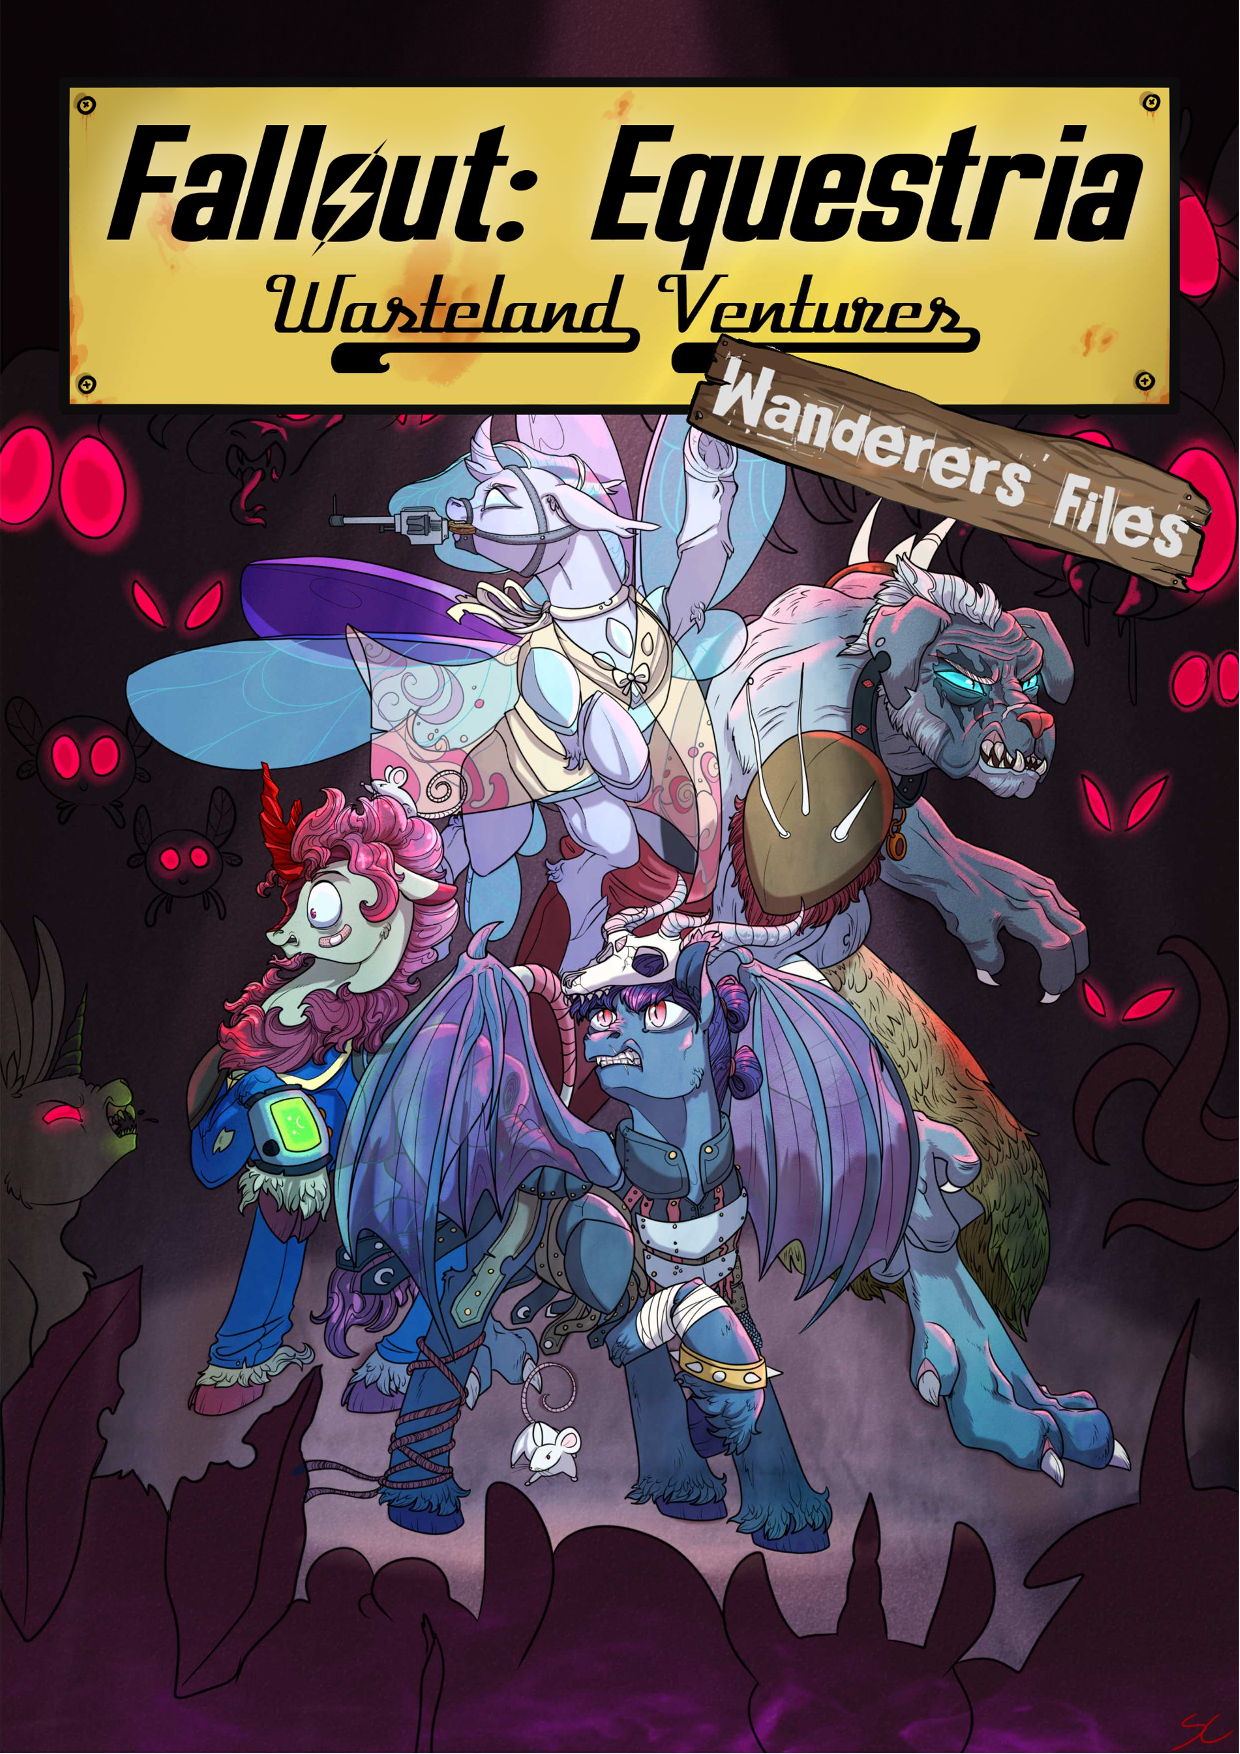
\includepdf[pages={1}]{WORD/COVER-WANDFILE.pdf}		
	\onecolumn
	\setcounter{page}{1}	
	\begin{center}
		Compiled by Waak, Kireanikin, LaPa, Miksu \& SourCherry
		
		10 AP rule basis by Yondalor
		
		Token HP \& Status rule bases by LZ
		
		\bigskip		
		\textbf{Playtesting and Advice:} LZ, Moonlight, Mittens, Kittyfluff, Ray\_Lionheart, f1r3w4rr10r, Tierney Kelly, Eden, Kendallkun, Pesian, Raven, dumbhat, GODOG, Borealis
		
		\bigskip
		\textbf{Cover and Graphics:} SourCherry
		
		\bigskip
		\textbf{Layout:} Waak \& SourCherry		

	\end{center}
	
	\vfill
	
	\begin{center}
		\textbf{Version 1.4.1}
		
		\emph{Last compiled on \thedate}
        
        \emph{\textbf{Contact:} wasteland-ventures@googlegroups.com}
     
	\end{center}	
    \begin{figure*}[bp]
		\centering
		
\includegraphics[width=3cm]{ART/ISA_Logo}
	\end{figure*}

	\twocolumn
	\tableofcontents


	\chapter{Introduction}
	
	The purpose of this book is to introduce new playable races into the system and everything they need to function, including their own brands of magic if applicable. In addition, the book holds in it the core races for the sake of having the full roster of playable characters present.
	
	The new magic systems were made to make some of the races a bit more unique and interesting.
	
	\chapter{Races}
	
	It wasn?t only ponies, zebras and griffons who survived the horrors of the apocalypse and t

	\section*{Abyssinian}
	\addcontentsline{toc}{section}{Abyssinian}
	A race of bipedal cats, abyssinians hail from a kingdom outside of Equestria?s borders. Hence why this race is rarely seen in the Wastes, as not many were present during the Last Day. However, while Equestria is now little more than a dead wasteland, Abyssinia has thrived, building their nation further. Yet, perhaps compelled by the feline curiosity, some make their way to the Equestrian Wasteland... 
	
	Though food and shelter is plenty in Abyssinia, the various magitech constructs they developed during the war are scarce and in bad shape, due to Abyssinia being low in magic-amplifying gems, which the Equestrian Wasteland still has in droves.
	
	Being feline in origin, abyssinians have the smooth, graceful moves of a cat, often bending and moving in ways ponies cannot. In addition to this, they have sharp claws on their paws that they can and often use to fend for themselves, and, much like bat ponies, abyssinians have slit pupils, and can see much better in dark than most equine species.
	
	The witches? black cats know tricks, as abyssinians wield magic like Unicorns. Their bodies and minds are also more adapted to magic, having greater resistance to arcane fatigue. 
	Instead of having a horn like the equine spellcasters, abyssinians use trinkets, wands and staffs to focus the magical energies they harness. Though abyssinians can cast magic without a catalyst -a magical artifact unique to each caster-, their delivery of the spell weakens considerably. 
	Traditionally, each abyssinian mage crafts their own catalyst, as it is believed that this allows the mage to channel their magic best. These catalysts are considered to reflect the mage?s virtue and personality. Should the catalyst break, they have to craft a new one (Thaumaturgy roll) with materials they feel reflect their personality the most.
	
	Abyssinians have the following racial abilities:
	\begin{description}
		\item[Eye in the Dark:] Abyssinians' eyes are made for hunting in the dark, letting them ignore 10 points of Visibility penalty caused by dark surroundings.
		\item[Sorcerer:] Abyssinians can tap into the same magical energy as unicorns do, giving them access to Unicorn Magic. Abyssinians can choose 3 Unicorn spells at character creation, and they have additional 10 Strain. However, they cannot learn new spells by level-up. They can only learn new spells by studying.
		\item[Cat-Alyst Caster:] Abyssinians perform their spellcraft through magical catalysts, such as wands, staffs, trinkets and jewelry. Abyssinians craft these artifacts from various mutant parts and junk. Casting spells without said catalyst removes the SPECIAL bonus from their spells? Potency, and adds +1 Strain cost.
		\item[Predator:] Abyssinians possess natural claws, giving them an extra dice to damage when using bare paws as Unarmed weapons.
	\end{description}
	
	\clearpage
	
	\section*{Bat Pony}
	\addcontentsline{toc}{section}{Bat Pony}	
	Bat ponies, though possessing same flight capabilities as pegasi, are otherwise a distinct race of their own. Most remaining tribes of bat ponies have kept to their ancestral homes deep in the cavernous Equestrian mountains. However, the Enclave and several mutated cave-dwellers have forced some tribes to come into view, so to speak.
	
	Some of the bat ponies were employed by Princess Luna as her personal guard and chariot-pullers. Perhaps due to both Princess Luna?s influence and their isolation from much of the Wasteland, the bat ponies? speak can sometimes sound archaic, though many do make a conscious effort to leave this habit into the past.
	
	Equipped with leathery bat wings -hence the name- and slit pupils, bat ponies are further divided from the other pony brethren by their relatively subdued and neutral color schemes of their mane and coat, though exceptions have been known to happen.
	
	Bat ponies? eyes react to light much like any dark-dwelling creature?s would, outwardly seeming quite cat-like, with their pupil changing size depending on amount of light the eye detects. Due to this, they have an excellent dark-vision, but color vision is quite poor.
	
	Bat ponies have the following racial abilities:
	\begin{description}
		\item[Cutie Mark:] Bat ponies have a special talent, giving them +5 to a skill when using their special talent.
		\item[Friend of the Night:] Bat ponies' eyes are well-versed for traversing in the dark, letting them ignore 10 points of Visibility penalty caused by dark surroundings.
		\item[Leathery Wings:] Bat ponies have wings and can fly. They can increase their flight capabilities by investing in Aerial Maneuvers.
		\item[Night Flight:] Bat ponies have a limited ability to perform Aerial Maneuvers. They can choose 2 at 1st level they have the requirements for, and gain a new one every 6 levels after (7th, 13th...). They have access to Wonderbolt Maneuvers.
	\end{description}

	\clearpage
	
	\section*{Brahmin}
	\addcontentsline{toc}{section}{Brahmin}
	
	Brahmin are the descendants of the mutated cows and bulls of wartime Equestria, most notable of their features being their two heads. As brahmin can be -though it is a rather rare instance- sentient, they often wear armor to protect themselves. And perhaps due to their large size and strong physique, they are excellent at hauling heavy weights.
	
	Out of the two heads brahmin possesses only one of the heads is sentient, the other has devolved to be little more than an animal working on instinct. Sometimes, the non-developed head can act on its own, but rarely does much harm on purpose.
	
	Though brahmin cows are more common sight in the Equestrian Wasteland, brahmin bulls also exist. Aside from lacking female brahmin?s bloated udders, they are similar in general appearance, only larger and perhaps a bit more hearty in stature. Both genders have horns, often in mismatched places, that continue to grow all throughout the brahmin?s life.
	
	Brahmin, much like the wartime cows and bulls, get along well with ponies, usually finding their stay in pony-centered cities leisurely and accommodated, even if it is technically a livestock stable...
	
	Brahmin have the following racial abilities:
	\begin{description}
		\item[Big Betsy:] Brahmin are able to pull heavier loads than most other species, and due to this, they do not suffer Encumbered-status from Heavy Armor that weight 15 kg or less.
		\item[Easy Load:] Brahmin have strong back, letting them carry much more than a pony could. Brahmin have +20 kg to their Carry Weight limit.
		\item[Fresh Pair of Eyes:] With additional head, brahmin are harder to surprise. They gain +10 to PER rolls against Stealth. However, the additional head comes at a price, being another Head that can be Crippled - thus brahmin may suffer from two Crippled heads, and their cumulative penalties.
	\end{description}
   
   	\clearpage
   	
   	\section*{Buffalo}
   	\addcontentsline{toc}{section}{Buffalo}
   
  	 Buffalo are the offspring of the tribals that roamed the southernmost plains and arid ranges of Equestria, especially around the old towns of Appleloosa and Dodge Junction. 
   
  	 Still holding tradition close to their hearts, buffalo maintain their identity strongly through their customs, such as an annual roam through a specific route in the mid-west Equestria, that has been roamed for countless generations. This adherence to tradition is still seen as odd in eyes of ponies, but most buffalo would agree that tradition makes them stronger and creates unity in a tribe.
   
   	Shamanism is strong with buffalo, being the only other race to communicate with spirits on a regular basis alongside zebra. Much like with zebra, this gift is highly respected in their communities as though many buffalo see and interact with spirits daily, but only a proper shaman can barter with them. Buffalo Shamans are often high in the social order, being the one to link the buffalo to their ancestry and to the nature around them and to give advice to the community by spirit counseling.
   
   	\textbf{Buffalo may take Shaman perks, if they possess Tribal Shaman trait.}
   
   	Buffalo have the following racial Abilities:
   	\begin{description}
	   	\item[Tribal Ancestry:] Buffalo, much like zebra, have a long history of shamanism in their tribes, with shamans holding much power and reverence. Buffalo have access to Spirit Magic and Tribal Shaman trait.
	   	\item[Easy Load:] Buffalo have strong back, letting them carry much more than a pony could. Buffalo have +20 kg to their Carry Weight limit.
	   	\item[Great Beast:] Buffalo are visibly larger than ponies, and have heavier builds. All buffalo are considered to be Size Category 1 at start, and they also gain an extra SPECIAL point to invest during character creation.
	   	\item[Healer:] Buffalo have a long history with medicine, from herbal mixtures to high-end chemistry. With a careful dosage, they can administer a Medical item twice, excluding  Doctor?s Bag and First Aid -kit.
	\end{description}

	\clearpage
	
	\section*{Changeling}
	\addcontentsline{toc}{section}{Changeling}
	
	One of the more evasive races in the Equestrian Wasteland, the changelings are shapeshifters whose original form resembles a thin insect and pony hybrid. Commonly seen as Equestria?s version of the boogeyman, due to their transformative magic hiding them in plain sight, many independent hives began to break out of their old molds after the Last Day; some for the better, some for the worse. Most settlements in Wasteland regard changelings with suspicion and fear, though there are exceptions.
	
	Changelings are unique in that they do not get the bulk of their nutrients from regular food -though eating material things is still somewhat useful during a shortage-, but rather they gather and eat emotions (Strain in this system) from ponies. To successfully steal emotions from them, they take the form of the pony?s loved one and feed off of the pony?s affections for that person. This is often preceded by getting rid of the original... 
	
	However, changelings are not perfect copies of the pony they?re posing as, only of their outward appearance, leaving their behavior something that a changeling has to study well to not get caught.
	
	Changeling hives rarely have contact with one another, causing a large chasm of differences from hive to hive, from their tactics to gather energy, to their general opinion on other creatures and to customs regarding social standing and cultural customs. Most commonly, the hive is ran by a changeling queen, a taller and more powerful creature than the common changeling. She makes the decisions in the hive, with or without input from her subjects. 
	
	Though changelings themselves have life-span of an average pony, the changeling queen can live hundreds of years, meaning that some of the changeling queens are old enough to remember the war and its cause and effect.
	
	Changelings have the following racial abilities:
	\begin{description}
		\item[Changeling Magic:] Changelings have a magic that is a mixture of Unicorn magic schools and their own unique spells. See Changeling Magic for details. Changelings start with Shapeshift for free, and 3 additional spells. They learn a new spell every 5 levels (6th, 11th...).
		\item[Contort:] Changelings have bug-like qualities, and they can contort their bodies in ways ponies cannot. They have +10 to Unarmed when grappling.
		\item[Strain Feeder:] Changelings feed off Strain of others because they do not regenerate Strain on their own. Strain can be given to the changeling willingly, or taken by force. See Changeling Magic for more details.
		\item[Chitinous Shell:] Changelings have thick chitin that gives them armor-like properties. This provides +5 DT when not wearing Heavy or Power armor.
	\end{description}
	
	\clearpage
	
	\section*{Crystal Pony}
	\addcontentsline{toc}{section}{Crystal Pony}
	
	Crystal ponies resemble earth ponies in outward appearance, but their shiny, crystal-like coat and gradiented manes set them apart from their earthy cousins. Hailing from the northern Crystal Empire, these ponies remained impartial to the conflict of the warring Equestria, though it was rumored that the empire was assisting them under the table, so to speak.
	
	The Crystal Empire?s ample defenses ensured that the stray bomb that hit near Yakyakistan would not cause as much harm on them as it did on the yaks, as the force field surrounding the empire kept much of the radiation at bay. However, the shield did not stop all of the magical fallout and the nuclear winter it brought with it from seeping in. For the first half a century, the Crystal Empire skies were sunny and the climate warm and the only sign of adversity were from an occasional feral ghoul here and there. 
	
	But soon it was found out that the power of the Crystal Heart was dwindling, allowing for more and more radiation to seep in, and the environment to grow colder. Emergency measures were taken to power the Crystal Heart, but they ultimately proved futile. As the radiation and nuclear winter engulfed the city, the crystal ponies found themselves with an empire unable to sustain itself properly. Despite this, the Crystal Empire still has some few stubborn individuals remaining to this day.
	
	Crystal ponies have the following racial abilities:
	\begin{description}
		\item[Cutie Mark:] Crystal ponies have a Special Talent, giving them +5 to a skill when using their special talent.
		\item[One with the Glow:] Though balefire is not the source of their mutation -that would be the Crystal Heart, an ancient magical artifact that gave off magical radiation much like a prototype megaspell-, crystal ponies are considered mutated. Due to this they have a boosted Poison Resistance of 15 and Radiation resistance of 10.
		\item[Abhorrent Past:] Crystal ponies are more in tune with their emotions, and this, coupled with the tyranny they suffered under king Sombra, has left them less capable of dealing with hardship. Their Insanity Chance is 25\% instead of 20\%. However, they did survive the tyranny and came back stronger: They have +1 to END to resist Mind-Control -status effect.
		\item[Ties to the Earth:] Much like their earth pony cousins, crystal ponies share their connection to earth. This gives them access to Earth Pony magic, and start with 3 Spells and gain a new one every 6 levels after (7th, 13th...).
	\end{description}

	\clearpage
	
	\section*{Deer}
	\addcontentsline{toc}{section}{Deer}
	
	Deer used to inhabit many of the Equestrian forests with their own kingdoms. Rather a  rare sight, as most ponies are used to seeing the deer?s unfortunate mutation, the Radstag. However, despite the popular notion that sane deer didn?t make it out of the magical fallout, some of the population did survive in a bunker of their own making.
	
	As the decades rolled on and the once lush forests either grew too hostile or died, the deer can sometimes be spotted in settlements surrounding their abandoned and overtaken kingdoms. However, the deer are still ruled by their community?s king, which is a hereditary position, unless the heir is too young or unfit to rule. 
	
	Outwardly, the deer are tall and lithe, their movements graceful and cautious. Around their necks, deer carry a cask, that can vary in shape and size. This cask contains a potion of their own making. However, unlike ponies, deer fare worse against the magical fallout, and due to this one can often find deer wearing a breather of sorts to protect their lungs from irradiated air.
	
	Deer?s Cask functions as a Quick Slot.
	
	Deer have the following racial abilities:
	\begin{description}
		\item[Blessing of the Green:] Deer utilize their magic with potions made from plants and earth from their surroundings, much like how zebra use alchemy to brew their potions. They have access to the Alchemy list, and start with 4 recipes with Skill Requirement of 30 or less.
		\item[Purity Flaw:] Deer are less tolerant of magical radiation and often require breathers to steer clear of harmful effects. Their Poison resistance is 15 and their Rad resistance is 0. However, they recover from wounds better than most races; they have +1 to Natural Healing Rate.
		\item[Quick Runner:] Deer are quick and agile creatures, reacting quickly to events happening around them, even when surprised. They have +2 to Initiative.
		\item[Sharp Horns:] Deer possess branching horns, giving them an extra die to damage when using horns as Unarmed weapons.
	\end{description}

	\clearpage
	
	\section*{Diamond Dog}
	\addcontentsline{toc}{section}{Diamond Dog}
	
	Though many diamond dogs have mutated into the fearsome hellhounds, some packs have eluded this fate. Retaining their form largely unchanged, diamond dogs are canine creatures that can walk on both four legs or two, giving them ample choices for weaponry.
	Diamond dogs have keen sense of smell and hearing, Much like their name implies, they have a great greed for gemstones. Due to this, they mostly inhabit caves and caverns, with strict hierarchy -a trait that remained in the mutated hellhounds- defining their way of life.
	
	Most packs of diamond dogs are led by an alpha, or if the alpha has deceased, by their companion, the matriarch. The alpha and matriarch both have a high social standing, with the alpha upholding and planning daily hunts, digs and gem hauls, as well as having the final say on who does what. The matriarch makes sure the community works well together, negotiating and separating individuals in a fight; she also handles issues in pup-caring. Much like pony societies, these packs can have good and bad leaders, resulting in vastly different packs. 
	
	However, despite their strict social hierarchy, members are free to roam if they want to, and can rise up in ranks through recognition as a valuable member. More often than not, the higher the rank, the more gemstones the diamond dog has on them. 
	
	Due to the wartime stories -of the second class citizenship diamond dogs had to endure in Equestria- that mothers pass on to their pups, diamond dogs do not mingle well with ponies; they are usually cautious and wary of any pony, and take a while to warm up to them. Other races however, rarely encounter this cautious behavior.
	
	Diamond dogs have long, thick claws that are primarily used for digging, and though they are not quite as strong and sharp as hellhound?s, they can dig through most common rock material and soil. They can also see fairly well in dark, though not quite as well as bat ponies or abyssinians. Diamond dogs are capable of eating plant material, but prefer fresh meat vastly over vegetables.
	
	Diamond Dogs have the following racial abilities:
	\begin{description}
		\item[Canine Claws:] Diamond dogs possess natural claws, giving them an extra die to damage when using bare paws as Unarmed weapons. In addition, said claws can pierce through meager armor, ignoring 5 DT.
		\item[Accustomed to Dark:] Diamond dogs? eyes are made for roaming their underground lairs, letting them ignore 5 points of Visibility penalty caused by dark surroundings.
		\item[All Ears:] Diamond dogs have sharp hearing, giving them +1 to PER when locating sneaking enemies, and +2 to Initiative. However, said hearing is sensitive to high-pitched sounds, giving them Moderate Distraction whenever subject to them. This includes whining from pony mares.
		\item[Underground Dweller:] Due to their habitat being self-dug caves and caverns, diamond dogs can ignore Difficult Terrain when traveling underground.
	\end{description}

	\clearpage
	
	\section*{Donkey}
	\addcontentsline{toc}{section}{Donkey}
	
	Though they?re hardly the next beauty queen winner, or even the runner-up, donkeys do have their place in the Equestrian Wasteland. Due to their sturdy nature, they?ve fared quite well despite the magical fallout. 
	
	Unlike ponies and various other magical creatures, donkeys are inherently magicless, making up for it with their tenacity and stubborn determination to see that their goals succeed. Donkey culture doesn?t vary much from pony culture, which is why donkeys often assimilate to society easily. 
	The only key difference is the donkey societies? more inward approach to strangers, not being quite as eager to befriend as ponies are. This usually means they?re slow to warm up to others they do not know well, but once one gains their trust, they prove a loyal friend through thick and thin. This of course, varies depending on individual.
	
	The most well-known settlement is Jennysburg, an old pre-war town mostly populated by donkeys, though a few other races from nearby have settled in, such as harpies. Reinforced and maintained with available scrap, the town sports a fairly standard Wasteland look to it, with every resource carefully maintained, harnessing what little the arid prairies have to offer.
	
	Donkeys have the following racial abilities:
	\begin{description}
		\item[Never Say Die:] Though donkeys lack the magical abilities of ponies, they make up for it by refusing to go down as quickly. Stubborn is the way of the donkey; Donkeys have an additional +2 HP.
		\item[Hit the Desert:] Donkeys origin from vast deserts in southern Equestria, though they have spread further in over the centuries. They however, retain their higher resistance to heat;, giving them a +10 DT against Fire damage and +1 END to resist Burning-status effect.
		\item[Beast of Burden:] Though donkeys are not as big and strong as brahmin or yaks, they can still haul impressive amounts of stuff on their backs. They gain +10 to their Carry Capacity.
	\end{description}

	\clearpage
	
	\section*{Harpy}
	\addcontentsline{toc}{section}{Harpy}
	
	Harpies are bipedal parrots with talons for legs and arms, and though rarely seen in the Equestrian Wasteland, some have made the derelict wastes their home, the situation of their homeland shrouded in mystery. 
	
	Unlike pegasi, griffon, hippogriffs and bat ponies, harpies are not able to fly or use cloud technology and they have no functional wings. Despite this, the harpies have spread far, found in the Southern Equestria?s cloud-covered mountains, to the coastal towns in the west coast, and the deep, wild jungles that surround the Badlands. The harpies have established some settlements in the Equestrian Wasteland, but these are more considered pit-stops rather than permanent settling, as harpies often move in near-nomadic fashion.
	
	Often armed with an adventurous spirit, they travel far and wide in search of experiences, even if it doesn?t always turn out so well for them. Because of this, it is quite common to see harpies with cybernetics that lack the refinement and smoothness of earth pony made cybernetics, but work just as well.
	
	The talons on the harpy?s legs and arms are sharp, and often used to fend for themselves if they run out of other weaponry. 
	
	Harpies have the following racial Abilities:
	\begin{description}
		\item[Bird of Prey:] Harpies possess natural claws, giving them an extra die to damage when using bare talons as Unarmed weapons.
		\item[Delicate Claws:] Harpies have slimmer talons than griffons do, allowing for more precise movement. They have +5 to Sleight and their Ready Item/Weapon costs 1 AP less, to a minimum of 1.
		\item[Broken but Functional:] Harpies take exceptionally well to adjusting their bodies with either permanent alchemical brews or cybernetics. They gain +2 to END when determining adjusting period after a new enhancement. This makes their formula 15 days $- ($END$+2)$.
		\item[Shock Resistant:] Perhaps due to their interest in mechanics and all things electric, harpies don?t find electric shocks quite as jump-inducing than most, shrugging off small shocks. Harpies have +1 to END to resist electricity-induced Stun-status effect.
	\end{description}
	
	\clearpage
	
	\section*{Hippogriff}
	\addcontentsline{toc}{section}{Hippogriff}
	
	Originating from Mount Aris, the hippogriff have become slightly more commonplace amongst the ponies after the Last Day. Much like deer, hippogriff remained impartial to the conflict, though unlike deer, this didn?t come back to bite them in the flank, as Mount Aris was spared from a direct hit.
	
	During the few hours that was the apocalypse, the hippogriff with their leader, Queen Skystar, disappeared underwater with the use of their magical pearl, transformed into seaponies. Perhaps due to this, hippogriffs/seaponies were spared from much of magical fallout that was eventually blown in their direction by wind. 
	
	Several generations later, the hippogriffs made their way up to the surface and began to traverse the Equestrian Wasteland.
	
	Hippogriffs have the following racial abilities:
	\begin{description}
		\item[Bird Brained:] Some say hippogriffs aren?t the sharpest pens in the sea. No, wait, that?s not how it went. Hippogriffs suffer -1 INT, but only have 10\% chance to gain Insanity.
		\item[Quick Runner:] Hippogriffs are agile creatures, mastering both traversing the sky and the land alike. They have +2 to Initiative.
		\item[Stable Wings:] Hippogriffs have wings and can fly. They can increase their flight capabilities by investing in Aerial Maneuvers.
		\item[Flexible Maneuvers:] Hippogriffs have a limited ability to perform Aerial Maneuvers. They can choose 2 at 1st level they have the requirements for, and gain a new one every 6 levels after (7th, 13th...). However, they can learn both Wonderbolt and Talon maneuvers.
	\end{description}

	\clearpage
	
	\section*{Kirin}
	\addcontentsline{toc}{section}{Kirin}
	
	The elusive and near mythical kirin are dragon-like equines with a single red branch-like horn protruding from their forehead, a fluffy mane that circles around their neck and dragon-like scales on their backs. They have cleft hooves and an ox-like tail as opposed to the pony-like tails. Like ponies, they come in a rainbow of colors.
	
	Discovered shortly before the war, kirin saw limited service at frontlines but made scary berserker-units using their Nirik-forms. They served mostly under pony units but few defectors served zebra legions. In exchange for their service under banner of Equestria, kirins got their own Stable near their village in Peaks of Peril. The Stable was almost finished before last day - it was fully operational but not fully reinforced. This quickly lead into some issues.
	
	The unfinished work resulted in an eventual breakage of the water systems in part of Stable; while not ultimately lethal for Stable as a whole, it caused some of the Stable?s water-supply to become tainted with the water from Lake of Silence. The magical properties of the lakewater rendered those who were exposed to it to hold their tongues and express their emotions with the bare minimum. 
	
	While they are not quite as silent and emotionless as pre-war Silent Ones, they still don?t speak much and barely show emotion even though they do still experience them. Most would consider their quiet, calm disposition unnerving, though they can also be stable and powerful mentally. Silent Ones almost never can enter Nirik state - one would need to be put in ultimately fatal position to achieve it.
	
	Despite mishaps, kirin Stable endured by virtue of tricky balance and philosophy outlined by its Overmare Autumn Blaze. Group therapies and mixing speaking kirin and Silent ones is encouraged while individual needs of each are fulfilled in their communities. Therefore Stable is divided in three areas: Speech, Silent and Common, where they can freely intermingle.
	
	Though still operational, eventually some kirins decided to begin exploring the Wastes around them and left the Stable.
	
	Kirins have the following racial abilities:
	\begin{description}
		\item[Elementalist:] Kirins have access to Elemental magic, closely resembling the arcane arts of Unicorns. Kirin start with 3 spells, 2 of their choice from the Kirin?s Spell list, and either Elemental Orb or Elemental Coat. They learn a new spell every 6 levels after (7th, 13th...). 
		\item[Fire and Fury:] Kirins can channel their anger, turning into a flaming demon-like equine dubbed Nirik. They can maintain this form for short periods of time, though prolonged exposure runs the risk of hurting their mental health. Kirins automatically enter Nirik form if they gain Enraged status.
		\item[Dragon Scales:] Being partly covered with scales, kirins gain an extra 5 DT when not wearing Heavy or Power armor.
		\item[Forest Walker:] Kirins ignore Difficult Terrain caused by forested areas or foliage.
	\end{description}

	\clearpage
	
	\section*{Minotaur}
	\addcontentsline{toc}{section}{Minotaur}
	
	Minotaurs hail from two side-by-side islands between the zebra nation and Equestria in the Luna ocean and have their own city states. These two city states, Pasiphaerium and Asterpolis, have had their differences from the first day of construction. It is no surprise that this feud escalated during the Great War, with both cities helping a different side of the conflict despite officially stated to be neutral. As both cities boasted impressive fleets of merchant ships and warships, as well as their leanings towards shrewd business practices, the cities grew richer than ever before.
	
	After the bombs fell, both Pasiphaerium and Asterpolis were saved from any direct attacks, but the apocalypse soon came to them as well; with most of the pony and zebra populous either dead or hidden inside Stables, the money sources went scarce. After the winds brought over the magical fallout, it was time for the minotaur to make their way to the mainlands, to seek out revenue before the ocean around them turned too hostile for travel.
	
	New cities, aptly named Nopos Pasiphaerium and Nopos Asterpolis, were constructed soon after, which hold a sizeable population of the minotaur. Both the old and new cities are ruled by their respective kings and queens.
	
	Minotaurs have the following racial abilities:
	\begin{description}
		\item[Great Beast:] Minotaurs are visibly larger than ponies, and have heavier builds. All minotaurs are considered to be Size Category 1 at start, and they also gain an extra SPECIAL point to invest during character creation.
		\item[Big n' Scary:] Though not all minotaurs are mean, most of them are intimidating by the virtue of their size and stature when compared to equines. Minotaurs have +5 to Intimidation against ponies and zebra.
		\item[Sound of Mind:] Perhaps due to minotaur culture, most minotaurs fare better in the face of traumatic experiences, putting the past happenings behind them faster through some well-placed self-assurance. Minotaurs? Insanity chance is 15\% instead of 20\%.
	\end{description}

	\clearpage
	
	\section*{Yak}
	\addcontentsline{toc}{section}{Yak}
	
	Originally from the frozen mountains near Crystal Empire, the yak kingdom of Yakyakistan was swayed to ally from both sides of the conflict, but ultimately the yaks allied with Equestria; some suspect the Ministry mare of MoM may have had a hoof in this. Though allies, yak forces were scarcely utilized during the war. And once the bombs dropped, the yak forces that still remained in Equestria headed home.
	
	Home, however, was not as it was remembered. A stray balefire missile had landed far too close for comfort to Yakyakistan, resulting in a nuclear winter the yaks could barely survive from. After much thought, stomping and screaming, a decision was made. The yaks would build a new Yakyakistan further south and settle there.
	
	The New Yakyakistan proved to be a sturdy, if a little on the small and simple side, settlement, and has remained from nearly as long as the Wasteland itself. Many of the yaks still hail from this city.
	
	Despite moving southward, yaks have not lost their thick, well-insulated fur or their strong disposition. Many yaks still hold tradition close to their heart, with their armors often taking cues from their history, though now made out of scrap metal. Many wartime armors have been passed down from generation to generation. Likewise, much of the yak fabric and culture -such as log-smashing or elaborate, earth-shattering dances- have been passed down from yak to the next.
	
	Yaks have the following racial abilities:
	\begin{description}
		\item[Thick Fur:] Yaks have a thick, insulating fur, giving them a +10 DT against Cold damage, and +1 END to resist Freezing.
		\item[Great Beast:] Yaks are visibly larger than ponies, and have heavier builds. All yaks are considered to be Size Category 1 at start, and they also gain an extra SPECIAL point to invest during character creation.
		\item[Hefty Guy:] Yak are able to pull heavier loads than most other species, and due to this, they do not suffer Encumbered-status from Heavy Armor that weight 15 kg or less.
	\end{description}

	\clearpage
	
	\chapter{Traits}
	
	These traits are additional traits for the races in this book in particular. This does not limit them from using the traits in the core rulebook.
	
	\section*{Battle Beast}
	\emph{\textbf{Yak-only trait}}
	
	Ancient yak battle chants have been passed down in your family for generations! You gain access to yak?s own elusive brand of magic; Battle Chants.
	
	Yak chants cannot be gained by level-up, and can only be learned. After all, one doesn?t know one song or a dance routine and suddenly intuitively know another after a while.
	
	Yaks start with two Chants at their disposal at Character creation.
	
	If the chanting character is attacked or subject of a Distract action, they have to roll Thaumaturgy to continue their chant. If successful, the chant continues, if failed, the chant ends. The effect of the chant is still held for the next turn, but the caster must start the chant again.
	
	Other yaks can assist Chanting by sharing the initial Strain cost, but the highest Strain cost must always be spent by the original caster. In addition, two separate chanters cannot sing different chants at the same time, as it creates a cacophony of sound. If this happens, neither chant?s effects happen due to the mixed sounds.
	
	\section*{Bodybuilder}	
	\emph{\textbf{Minotaur-only trait}}
	
	Okay, so you?re not the sharpest tool in the shed, not by a long shot. But what does that matter when you crush bones as easy as a grape? Your unarmed strikes always have a base 10\% chance of causing Crippled, but your INT is lowered by 2.
	
	\section*{Carnivore/Vegetarian}
	
	Food is good and tasty, but some food tastes better for you than others. You have a bit more distinct palate than most, and turn up your nose at your unfavorite, be it steamed beans or bacon bits.
	
	A character with Carnivore -trait gains +1 extra HP from any meat, be it raw or cooked. Any vegetables suffer a -1 to HP they give upon eating. A character with Vegetarian -trait gains +1 extra HP from any vegetable, but any meat suffers -1 to HP they give upon eating.
	
	A character cannot have both versions of the trait.
	
	\section*{Clovenless Upbringing}
	\emph{\textbf{Buffalo-only Trait}}
	
	As long as you can remember, you?ve had split hooves unlike your brethren, and maybe a larger size, nice twin horns, and a lot more oomph on your back. You?ve clearly been raised outside of your herd of buffalo but that didn?t slow you down. Instead, you?ve been raised by ponies.
	
	You grew up with more grace to your steps and precise use of your cloven hooves, giving you +1 AGI. However, that prevented you from being trained to the sturdy nature of buffalo. You lose the extra 20kg to your Carry Weight.
	
	\section*{Convincing}
	\emph{\textbf{Changeling-only trait}}
	
	Your disguises aren?t quite as numerous as most changelings?, but you?re leagues more convincing in them, knowing them like the back of your hole-y hoof.
	
	At character creation, you have 5 forms available to you, decided by you. Your Shapeshift is only limited to these 5 forms. Otherwise, Shapeshift-spell works as normal. You gain +2 to CHA when under scrutiny from others, and you gain a +5 to either Barter, Diplomacy or Intimidation.
	
	\section*{Changed -Ling}
	\emph{\textbf{Changeling-only trait}}
	
	On your travels you found the secret to not starving to death, loving yourself and others! Cheesy? Yes, but also useful - and nutritious. This doesn?t necessarily make others any less suspicious of you, however.
	
	You gain the Changed-reward Perk for free, however, there is notable downside to this - you only know two spells and Shapeshift at start and your \textbf{Intimidation}, \textbf{Sleight} and \textbf{Sneak} skills are lowered by 5.
	
	\section*{Echolocation}
	\emph{\textbf{Bat Pony -only trait}}
	
	You have a gift, rare amongst your kin; you can use high-pitched screaming to locate your surroundings. You gain +1 to your PER when using this method to check for your surroundings. While most other races and mutants cannot hear you, some certainly can - including bloodwings, dogs, diamond dogs and hellhounds.
	
	\section*{Fragile Beauty}
	\emph{\textbf{Crystal Pony -only trait}}
	
	You surpass even diamonds in the contest of beauty, and roses look like wilted weeds in your presence. Your shimmering, crystal coat gives you a +2 to CHA, but while your crystal hide is indeed fair, what it isn?t is durable; in exchange of gained CHA, you lose 2 HP. 
	
	\section*{Hot Blooded}
	\emph{\textbf{Yak-only trait}}
	
	You?re a force to reckon with once you get badly hurt. When reaching a Pain Threshold, you gain 4 extra dice to the damage you deal. However, your PER and AGI drop by 2 until you?re healed.
	
	\section*{Junktown Engineer}
	\emph{\textbf{Harpy-only trait}}
	
	While most harpies are seafarers and adventurers, you have a special knack for all things mechanical. Your best friends are the old world tech that those same seafarers and adventurers pull from the depths of the sea and from ancient ruins. 
	
	You can build inventions without Schematics, but upon first use the item needs to pass a LCK check. On a failed roll, the invention falls into pieces. If the item is a weapon, a critical failure requires another LCK check to see if it falls apart. In addition, the GM can request the character to check if their invention still works.
	
	\section*{Lamenter of Forest}
	\emph{\textbf{Deer-only trait}}
	
	You?re part of one of the largest communities of the deer, a mixture of culture and religion focused on and around the old way of life; your home is one of the many dying forests of the Equestrian Wasteland, hid away from outsiders. The forests you call home are a treacherous and poisonous environment, and it was your daily life for a long while. 
	
	Your \textbf{Melee}, \textbf{Thaumaturgy} and \textbf{Survival} skills have a +5 bonus on rolls, but your \textbf{Diplomacy}, \textbf{Firearms} and \textbf{Mechanics} skills suffer a -5 penalty on rolls.
	
	\section*{Long Distance Spellcaster}
	\emph{\textbf{Abyssinian-only trait}}
	
	You can throw your spells further than most. You have +2 to Potency when determining range of the spell. However, your spells also tire you out faster, as these spells have a +2 to Strain cost if flung beyond their normal range.
	
	\section*{Salty Blood}
	\emph{\textbf{Hippogriff-only trait}}
	
	You inherited a little, tiny sliver of the pearl?s magic through your ancestors, transforming you into a seapony when in contact with large bodies of water, both fresh and salty.
	
	When in seapony form, the hippogriff is immune to drowning, and can utilize their Aerial Maneuvers underwater (if they can plausibly be performed), and their flight speed translates to their Swim Speed underwater.
	However, in this form their Poison resistance drops by 5, and they cannot make Sleight or Lockpick checks.
	
	\section*{Scholar}
	\textbf{This trait requires the character has access to a form of magic.}
	
	You?ve spent most of your life shunning the outside world to practice your magic. This gives you an extra spell/maneuver at the start, but lowers your Diplomacy and Barter skills by -5.
	
	\section*{Small Breed}
	\emph{\textbf{Diamond dog -only trait}}
	
	Most Diamond dogs are kinda big and scary-looking. You?re the opposite of that, small and almost cuddly in your looks. Until you get angry and show them the meaning of ?Small Dog Syndrome? and nothing short of Tartarus-fuelled fury.
	
	Your Size Category is -2, but your Intimidation skill drops by -10. 
	
	This trait cannot be taken with \textbf{Small Frame} or \textbf{Large Frame} traits.
	
	\section*{Silent One}
	\emph{\textbf{Kirin-only trait}}
	
	You don?t speak much, nor would most call you the most expressive of kirins. Whether by accident or with intent, you?ve been in touch with the Lake of Silence?s magical water which has caused your state.
	
	You cannot access your Nirik-form, and you suffer -5 on your Barter and Diplomacy skills.
	
	On the other hoof, you are extremely hard to read, meaning you?re going to rake in all the caps in any game of poker... You also have total immunity to Enraged-status, and +1 END against Mind-Control -status effect.
	
	\section*{Split Personality}
	\emph{\textbf{Brahmin-only trait}}
	
	As long as they agree, two heads are better than one. Yours might do that, might not. 
	
	Both heads of a brahmin are sentient, able to think separately, while still functioning. You gain +1 INT and +1 to Initiative but you suffer -1 CHA and -1 to NPC disposition. Also, your actions and interactions are split between two personalities, making you occasionally clash with oneself.
	
	\textbf{This Trait is subjected to GM?s approval.} It can be played with two players sharing a character, and thus requires co-operation.
	
	\section*{Too Stubborn to Die}
	\emph{\textbf{Donkey-only trait}}
	
	You are the shining beacon of donkeys? stubbornness, as you refuse to even go down nice and easylike. Character with this trait has an extra turn to be healed after their HP hits 0. 
	
	Downside is they suffer a little bit more when their body begins to show pain before death; When rolling Pain Threshold penalties for this character, the GM adds a +1 to the roll. This +1 has no effect when it goes over 10, giving the character the biggest penalty on the list.
	
	\section*{Unidexterous}
	\emph{\textbf{Reserved for Abyssinians, diamond dogs, harpies or minotaurs}}
	
	As it turns out, you greatly prefer one paw or talon over the other. You gain +5 to hit to a combat skill when using one-handed guns (pistols, revolvers, SMG?s) or melee weapons. 
	
	However, when using two-handed weapons (Rifles, shotguns, two hoof swords and spears), your combat skill drops by 5.
	
	\clearpage
	
	\chapter{Unique Magic}
	
	\section*{Changeling Magic}
	\addcontentsline{toc}{section}{Changeling Magic}
	
	\subsection*{Learning Spells}
	Changelings have a magic that is a blend of Unicorn magic and their own unique spells. Changelings start with Shapeshift for free, and 3 additional spells. They learn a new spell every 5 levels (6th, 11th...).
	
	Changelings have access to \textbf{General}, \textbf{Illusion}, \textbf{Perception} and \textbf{Transmutation} magic schools from Unicorn magic spell list, found in \emph{\textbf{Magic Codex}}.
	
	Like unicorns, changelings can learn spells outside of gaining a level. When studying to learn a new spell, they need 4 successful SPECIAL rolls, determined by the Magic School. They can only roll for learning once per day and failed rolls do not negate successes. Once the changeling has rolled 4 successes, she has gained a new spell. A teacher lowers the required amount of successes to 2.
	
	\subsection*{Use of Strain}
	Changelings do not have Strain recovery from rest like other races do, and must take it -either willingly given or forcibly taken- from other creatures. Changelings cannot, in most cases, drain all Strain out of target in one go. They can drain 5 Strain from a single target unless using the Create Cocoon -spell, which is a notable exception. 
	
	If the Strain is given willingly, no roll is required. Forcibly taking Strain from other characters requires an opposed CHA roll. If the changeling loses the opposed roll, they recover no Strain and, in case they are disguised, have their disguise blown by the target.
	
	Having the target restrained in some way, such as tied up, gives the changeling a +1 to CHA for the purpose of forcibly taking Strain from the target.
	
	Though changelings do not regenerate Strain on their own, their maximum Strain does increase alongside other races by +5 Strain every 5th level.
	
	\subsection*{Breaking the Disguise}
	Changelings? very being is tied to one spell in particular, the Shapeshift spell. This spell allows them to take the form of another creature with a well-crafted illusion that takes use of all the senses. 
	
	However, particularly perceptive creatures can see through the disguise. Should this happen, the changeling character and the suspicious individual roll opposed CHA vs. PER. If the changeling is victorious, her cover is not blown, but if she loses the opposed roll, her cover is blown. What happens next is up to the GM to decide.
	
	In addition, sudden state of unconsciousness breaks the disguise immediately; a sleeping changeling can uphold their disguise, but being knocked out from a blow to the head breaks the illusion.
	
	\subsection*{Changeling Spells}
	\addcontentsline{toc}{subsection}{Changeling Spells}
	
	
	
	
	
	
	
	
	
   
\end{document}